% !TEX program = lualatex
%!TEX TS-program = lualatex
\documentclass[12pt,a4paper]{article}
\usepackage{fontspec}
\usepackage{polyglossia}
\setdefaultlanguage{polish}
\usepackage{geometry}
\geometry{margin=2.1cm}
\usepackage[table]{xcolor}
\usepackage{longtable}
\usepackage{array}
\usepackage{booktabs}
\usepackage{enumitem}
\usepackage{ragged2e}
\usepackage{graphicx}
\usepackage{float}
\definecolor{tableHeader}{HTML}{E8EEF7}
\definecolor{tableStripe}{HTML}{F7F9FC}
\newcolumntype{L}[1]{>{\RaggedRight\arraybackslash}p{#1}}
\newcolumntype{C}[1]{>{\Centering\arraybackslash}p{#1}}
\renewcommand{\arraystretch}{1.22}
\setlength{\tabcolsep}{4pt}
\setlist[itemize]{leftmargin=*, itemsep=2pt, topsep=2pt}
\setlength{\parindent}{0pt}
\setlength{\parskip}{6pt}
\emergencystretch=3em
\sloppy
\begin{document}

\section*{Raport ze sprintu nr 5 - Calisia Banking App}
Data raportu: 25.05.2026

Okres sprintu: 20.05 - 25.05.2026

Product Owner / Scrum Master: Michał Nuckowski

\subsection*{Lista osób}
\begin{itemize}
\item Kubryn Jeremiasz
\item Łaszuk Jakub
\item Makarevich Ksenia
\item Nuckowski Michał
\item Ruczyńska Nikola
\item Wołczko Jakub
\item Olszewski Dawid
\end{itemize}

\subsection*{Product Owner i Scrum Master sprintu}
Michał Nuckowski

\subsection*{Lista historyjek na sprint}
\begingroup
\footnotesize
\rowcolors{2}{tableStripe}{white}
\begin{longtable}{@{}C{0.08\textwidth}L{0.62\textwidth}C{0.10\textwidth}L{0.12\textwidth}@{}}
\toprule
\rowcolor{tableHeader}
\textbf{Kod} & \textbf{Historyjka} & \textbf{SP} & \textbf{Status} \\
\midrule
\endfirsthead
\toprule
\rowcolor{tableHeader}
\textbf{Kod} & \textbf{Historyjka} & \textbf{SP} & \textbf{Status} \\
\midrule
\endhead
S5-01 & Endpoint dashboardu klienta & 8 & Done \\
S5-02 & Kafelki produktów i saldo łączne w UI & 5 & In Progress \\
S5-03 & Projekcje zdarzeń domenowych do read modelu & 13 & Done \\
S5-04 & Oś czasu zdarzeń w dashboardzie & 5 & Done \\
\bottomrule
\end{longtable}
\endgroup

\subsection*{Podsumowanie sprintu}
Cel sprintu: Dashboard i model odczytowy. Pokazanie klientowi aktualnego stanu produktów (kont, kart i kredytów), salda łącznego i ostatnich zdarzeń w panelu bankowości.

Zakres sprintu obejmował 4 historyjki o łącznej estymacji 31 SP - z czego 3 historyjki zostały dowiezione ze statusem Done, a 1 z statusem In Progress, dlatego osiągnięta prędkość sprintu wyniosła 26 SP.

Dostarczono dashboard klienta oparty o model odczytowy: saldo łączne, kafelki dla kont bankowych oraz oś czasu zdarzeń. Nie udało się w pełni zaimplementować kafelków dla kart oraz kredytów.Projekcje aktualizują dane widoczne w panelu po operacjach finansowych.

Sprint połączył logikę domenową z widokiem klienta. Użytkownik otrzymał czytelny obraz swoich produktów i operacji, a zespół potwierdził sens rozdzielenia write modelu i read modelu.

\subsubsection*{Najważniejsze rezultaty}
\begin{itemize}
\item Dodano endpoint dashboardu klienta.
\item Wyświetlono kafelki dla kont bankowych i saldo łączne.
\item Wdrożono projekcje zdarzeń domenowych.
\item Udostępniono oś czasu ostatnich zdarzeń.
\end{itemize}

\subsection*{Retrospekcja sprintu}
Sprint pokrywał się dla wielu członków zespołu z zjazdem na Uczelni, co wymagało elastyczności w planowaniu i komunikacji. Mimo tego udało się utrzymać stabilny poziom energii i dostarczyć kluczowe funkcjonalności, chociaż nie wszystkie planowane zadania zostały ukończone. Retrospekcja pokazała, że synchronizacja między modelem zapisu, outboxem, projekcjami i widokiem frontendu jest kluczowa i wymaga testów integracyjnych obejmujących cały przepływ danych.

\subsubsection*{Co się udało}
\begin{itemize}
\item Udało się połączyć zdarzenia domenowe z modelem odczytowym.
\item Dashboard zaczął prezentować klientowi realną wartość produktu.
\item Zespół utrzymał testy integracyjne dla przepływu danych.
\item Frontend otrzymał spójny kontrakt do prezentacji produktów i zdarzeń.
\end{itemize}
\subsubsection*{Poziom energii zespołu}
Średni poziom energii zespołu: 4,1/5.

Energia zespołu była stabilna. Największym wyzwaniem była synchronizacja modelu zapisu, outboxa, projekcji i widoku frontendu. Utrudnieniem było pokrywanie się sprintu ze zjazdem na Uczelni, ale paradoksalnie miało to bardzo pozytywny wpływ na komunikację między członkami zespołu.

\subsubsection*{Czego udało się nauczyć}
\begin{itemize}
\item Zespół nauczył się praktycznego wykorzystania projekcji read modelu.
\item Outbox pomaga ograniczyć ryzyko niespójności między zapisem i odczytem.
\item Dashboard wymaga testów obejmujących zarówno API, jak i dane po operacjach finansowych.
\item Niektóre zadania, takie jak kafelki dla kart i kredytów, mogą wymagać więcej czasu niż pierwotnie zakładano.
\end{itemize}
\subsubsection*{Wnioski i działania na kolejny sprint}
\begin{itemize}
\item Rozszerzać testy integracyjne o scenariusze po kilku operacjach finansowych.
\item Dopisywać przypadki Bruno pokazujące pełną ścieżkę do dashboardu.
\item Przy przelewach od razu sprawdzać wpływ operacji na read model.
\item Doprecyzować estymacje dla zadań związanych z kartami i kredytami, aby lepiej planować zakres sprintu.
\end{itemize}

\subsection*{Następny sprint}
Product Owner / Scrum Master w następnym sprincie: Dawid Olszewski

Główny cel następnego sprintu: Przelewy własne i zewnętrzne. Pozwolenie klientowi na wykonywanie przelewów oraz odzwierciedlanie ich w saldach i historii.

\subsection*{Zrzuty ekranu}

\begin{figure}[H]
    \centering
    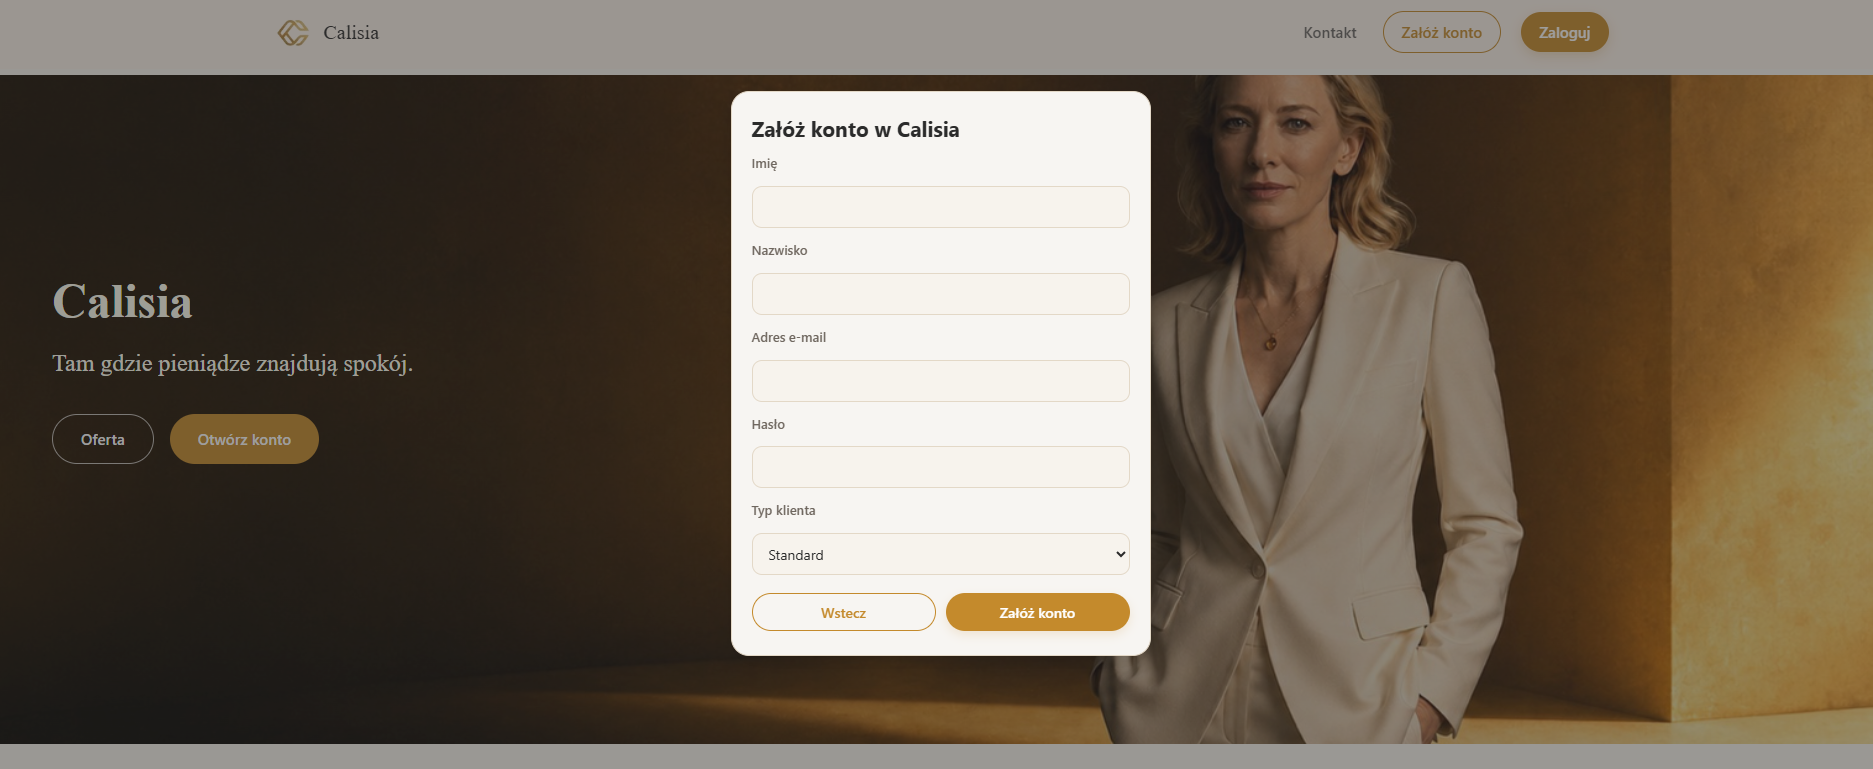
\includegraphics[width=0.95\textwidth]{assets/01_rejestracja.png}
    \caption{Rejestracja użytkownika.}
\end{figure}

\begin{figure}[H]
    \centering
    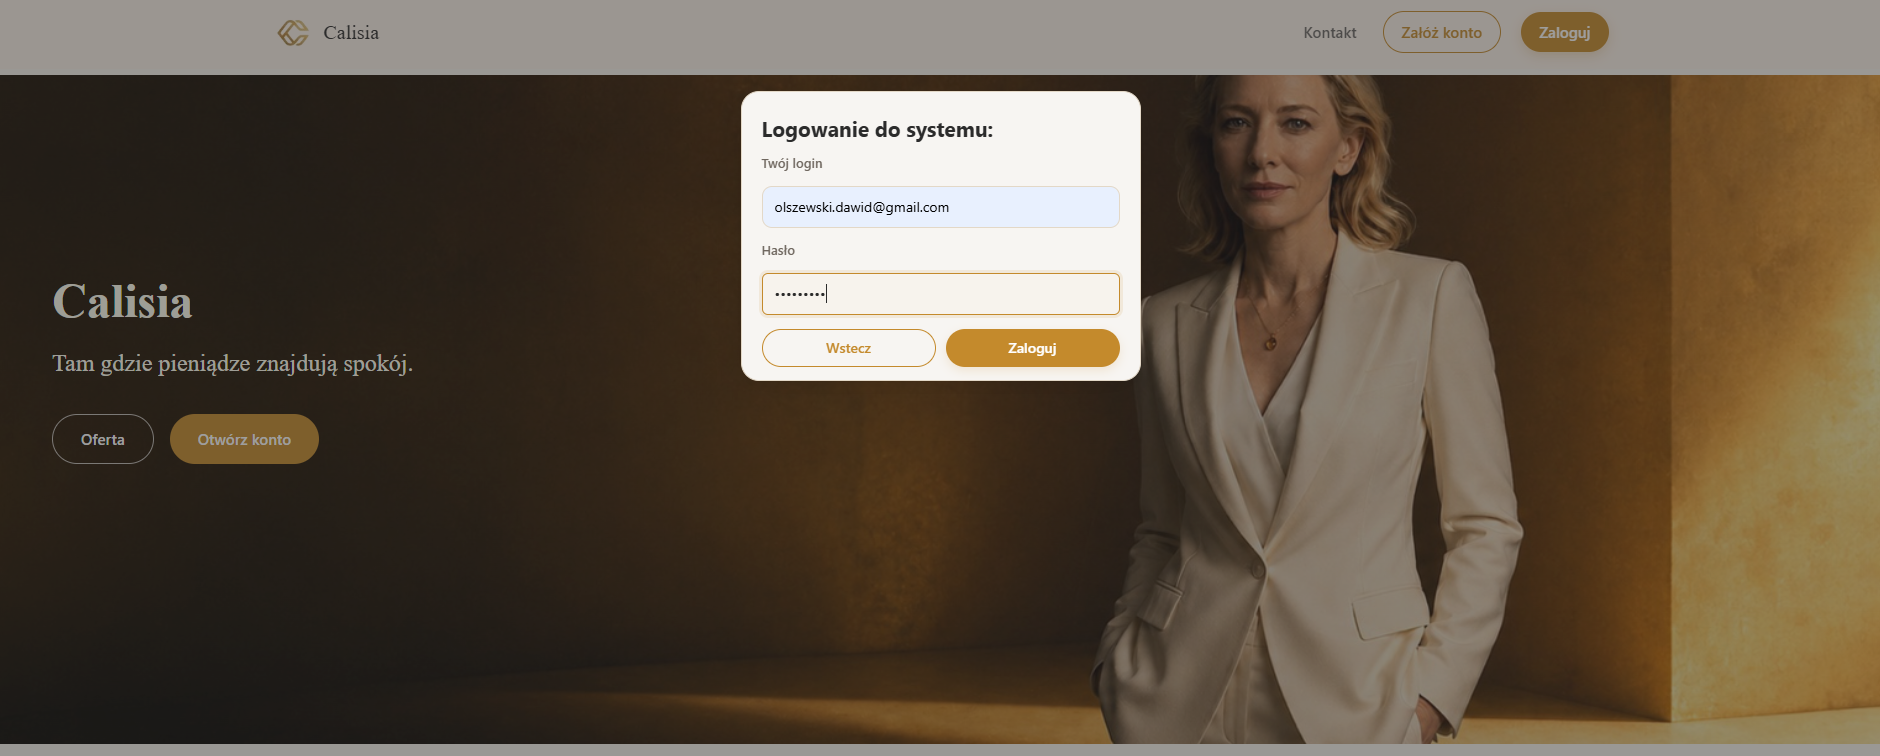
\includegraphics[width=0.95\textwidth]{assets/02_logowanie.png}
    \caption{Logowanie użytkownika.}
\end{figure}

\begin{figure}[H]
    \centering
    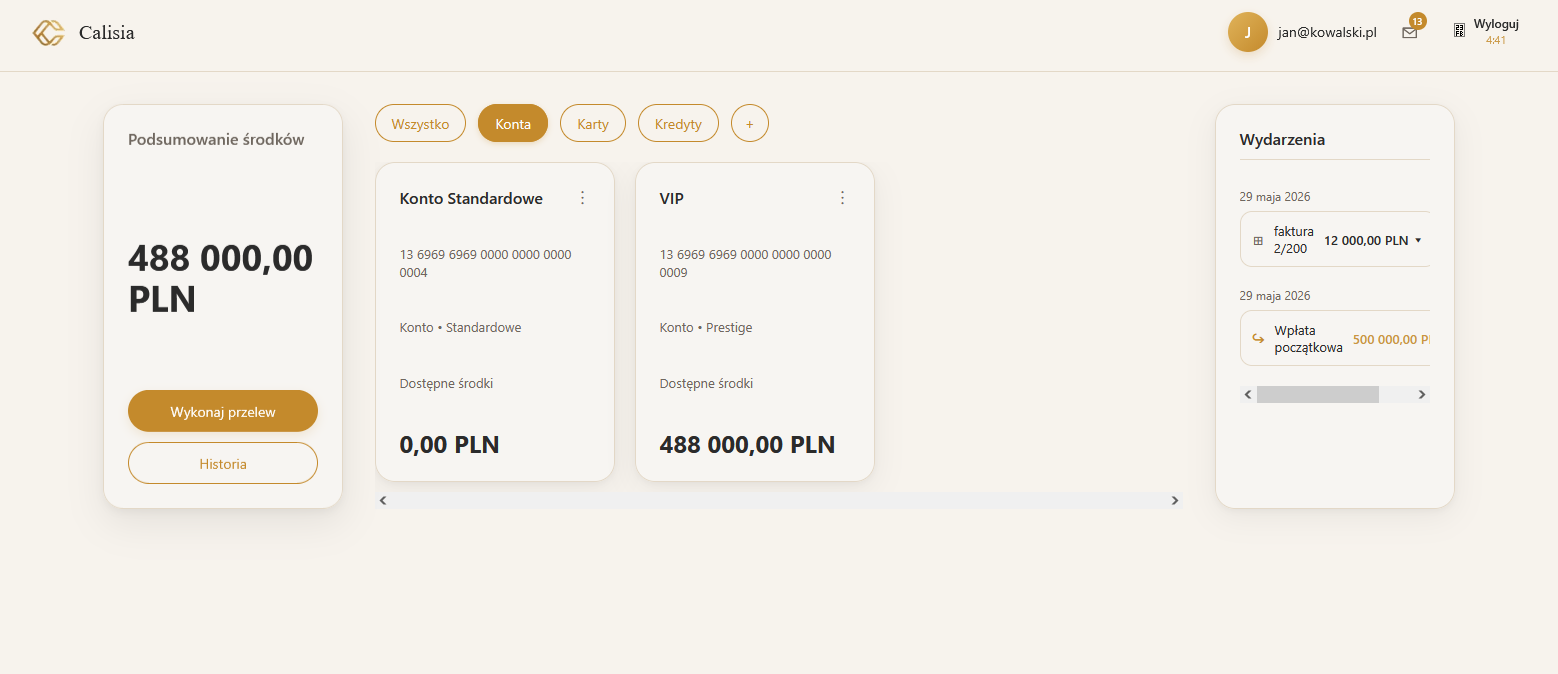
\includegraphics[width=0.95\textwidth]{assets/03_dash.png}
    \caption{Dashboard użytkownika.}
\end{figure}

\begin{figure}[H]
    \centering
    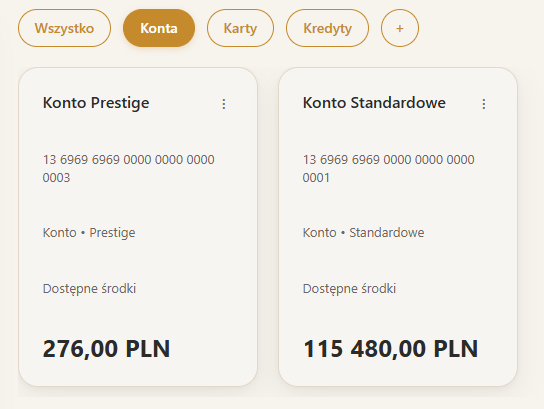
\includegraphics[width=0.95\textwidth]{assets/04_konta.png}
    \caption{Konta użytkownika.}
\end{figure}

\end{document}
